\chapter{Gimbal Control}
\label{chp:chapter2}
\graphicspath{{figures/}{figures/chapter2/}}
Gimbal is a widely used device for flying drones with camera because it stabilizes the camera from vibration and movement of the platform. Stabilizing camera is important in order to take high-quality, smooth videos and photos. For this reason, most of high-end commercial drones are equipped with gimbal. For autonomous systems, gimbal becomes more important because it adds maneuverability to the camera to provide with more visual awareness and to keep the object of interest in the camera field of view. There are two ways to keep the object of interest in the camera field of view: First, when we know the relative location of the target to the camera. Second, when we know the target location in image. For many practical applications, it is not feasible to assume that we know the target location in global frame. Thus, image-based gimbal control becomes more practical and realistic way to achieve the goal. In this chapter, we introduce multiple image-based gimbal control schemes.

\begin{figure*}[t]
    \centering
    \begin{subfigure}[t]{0.5\textwidth}
    	\centering
    	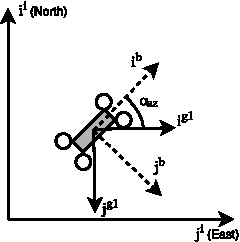
\includegraphics[width=2in]{images/chapter2/gimbal1_frame}
    	\caption{Top view to show the relationship between body frame and gimbal-1 frame}
    \end{subfigure}%
    ~ 
    \begin{subfigure}[t]{0.5\textwidth}
    	\centering
    	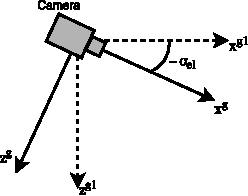
\includegraphics[width=2in]{images/chapter2/gimbal_frame}
    	\caption{Side view to show the relationship between gimbal-1 frame and gimbal frame}
    \end{subfigure}
    \caption{Frames of interest: body frame, gimbal-1 frame, and gimbal frame}
    \label{gimbal_frame}
\end{figure*}

\section{Angle Commanding Gimbal Control}
\subsection{Coordinate Frame Convention and Projective Camera Geometry}
Before giving a detailed explanation of the gimbal control algorithms, it is worth to set up the coordinate frame convention and projective camera geometry. Note that the coordinate frame convention here is following the convention from chapter 13 of \cite{beard2012small}. We assume that the origins of gimbal and camera frames are on the same point as the center of mass (COM) of the UAV. This is a reasonable assumption because the distance between camera, gimbal and the UAV COM is negligible compared to the distance between the UAV COM and the target. Also, note that all coordinate frames and the direction of rotation follow the right-hand rule. There are four frames of interests: the body frame of the UAV denoted by $\mathcal{F}^b=(i^{b}, j^{b}, k^{b})$, the gimbal-1 frame denoted by $\mathcal{F}^{g1}=(i^{g1}, j^{g1}, k^{g1})$, the gimbal frame denoted by $\mathcal{F}^{g}=(i^{g}, j^{g}, k^{g})$, and the camera frame denoted by $\mathcal{F}^{c}=(i^{c}, j^{c}, k^{c})$. The gimbal-1 frame can be obtained by rotating $\mathcal{F}^b$ about $k^{b}$ axis by $\alpha_{az}$ which we call the gimbal azimuth angle. The gimbal frame can be obtained by rotating $\mathcal{F}^{g1}$ about $j^{g1}$ axis by $-\alpha_{el}$ which we call the gimbal elevation angle. The negative sign is added because gimbal tilts down where tilting up is positive rotation (See Fig. \ref{gimbal_frame}). The camera frame is following the same direction as the pixel value grows in image with $k^{c}$ axis pointing straight out of the camera sensor. Thus, the rotation from body frame to gimbal-1 frame can be expressed as

\begin{equation}
R^{g1}_b(\alpha_{az}) = \begin{bmatrix}
\cos\alpha_{az} & \sin\alpha_{az} & 0 \\
-\sin\alpha_{az} & \cos\alpha_{az} & 0 \\
0 & 0 & 1
\end{bmatrix}.
\label{eq1}
\end{equation}
Similarly, the rotation from gimbal-1 frame to gimbal frame can be expressed as 
\begin{equation}
R^g_{g1}(-\alpha_{el}) = \begin{bmatrix}
\cos(-\alpha_{el}) &  0 & \sin(-\alpha_{el})\\
0 & 1 & 0 \\
-\sin(-\alpha_{el}) & 0 & \cos(-\alpha_{el})
\end{bmatrix}
= \begin{bmatrix}
\cos\alpha_{el} &  0 & -\sin\alpha_{el}\\
0 & 1 & 0 \\
\sin\alpha_{el} & 0 & \cos\alpha_{el}
\end{bmatrix} = R^g_{g1}(\alpha_{el}).
\label{eq2}
\end{equation}
The last two equations from the equation \ref{eq2} allow to use just the angle between $i^{g1}$ and $i^{g}$ without having to add the negative sign before the angle value. 
Combining the equations \ref{eq1} and \ref{eq2}, we get the rotation from the body frame $\mathcal{F}^b$ to gimbal frame $\mathcal{F}^{g}$ 
\begin{equation}
R^{g}_b(\alpha_{az}, \alpha_{el}) = R^g_{g1}(\alpha_{az})R^{g1}_b(\alpha_{el}) =
\begin{bmatrix}
\cos\alpha_{el}\cos\alpha_{az} & \cos\alpha_{el}\sin\alpha_{az} & -\sin\alpha_{el} \\
-\sin\alpha_{az} & \cos\alpha_{az} & 0 \\
\sin\alpha_{el}\cos\alpha_{az} & \sin\alpha_{el}\sin\alpha_{az} & \cos\alpha_{el}
\end{bmatrix}.
\label{eq3}
\end{equation}

\begin{figure}[t]
	\centering
	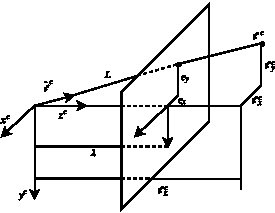
\includegraphics[width = 3.5in]{images/chapter2/camera_frame}
	\caption{Camera frame and visual aid for projective camera model}
	%
	\label{camera_frame}
\end{figure}

The camera frame, often referred as optical frame, is following the common computer vision convention: $i$-axis grows to the right, $j$-axis grows to the bottom and $k$-axis grows to the out from the camera optical sensor (See Fig. \ref{camera_frame}). Thus, the rotation from the gimbal frame to the camera frame is fixed once a camera is mounted on a gimbal and is given by 
\begin{equation}
R^{c}_g =
\begin{bmatrix}
0 & 1 & 0 \\
0 & 0 & 1 \\
1 & 0 & 0
\end{bmatrix}.
\label{eq4}
\end{equation}

The basic idea of the projective camera model is that the real 3D world is projected onto a 2D image plane that is orthogonal to $k^c$ axis with distance being the focal length $f$ from the origin of the optical axis (See Fig. \ref{camera_frame}). Because of this projection, we lose the distance information to the target which has introduced wide research problems in computer vision and estimation area. 
The focal length of the camera is the distance between optical sensor and lens, and it can be obtained through camera calibration. Since common camera calibration gives the focal length in the unit of pixel, the camera's field of view angle ($M$) can also be obtained as
\begin{equation}
M=2\tan^{-1}\bigg(\frac{\epsilon_{max}}{f}\bigg)
\end{equation}
where $\epsilon_{max}$ is the maximum pixel value from the center of the image. 

\subsection{Derivation}
Let the unit vector from the camera frame origin to the target (ie. the line of sight vector or LOS vector) in the camera frame be defined as 
\begin{equation}
\hat{\ell}^c=\frac{1}{L}
\begin{pmatrix}
\epsilon_x \\
\epsilon_y \\
f
\end{pmatrix}
=\frac{1}{\sqrt{\epsilon_x^2+\epsilon_y^2+f^2}}
\begin{pmatrix}
\epsilon_x \\
\epsilon_y \\
f
\end{pmatrix}
=\begin{pmatrix}
\hat{\ell}_x^c \\
\hat{\ell}_y^c \\
\hat{\ell}_z^c
\end{pmatrix}.
\label{unitlos}
\end{equation}
Angle commanding gimbal control algorithm computes the gimbal azimuth and elevation angles that would make the optical axis align with the unit LOS vector. By transforming the unit LOS vector (\ref{unitlos}) into the body frame, we get the desired optical axis direction as shown below
\begin{equation}
\hat{\ell}^b=R_{g}^b R_{c}^g\hat{\ell}^c.
\label{unitbodylos}
\end{equation}
By equating the equation (\ref{unitbodylos}) to the unit optical axis vector transformed into the body frame, we can compute the desired azimuth and elevation commands as
\begin{align}
\hat{\ell}^b&=\begin{pmatrix}
\hat{\ell}_x^b \\
\hat{\ell}_y^b \\
\hat{\ell}_z^b
\end{pmatrix}=R_{g}^b(\alpha_{az}^d, \alpha_{el}^d) R_{c}^g\begin{pmatrix}
0 \\ 0 \\ 1
\end{pmatrix}
\\&=\begin{bmatrix}
\cos\alpha_{el}^d\cos\alpha_{az}^d & -\sin\alpha_{az}^d & \sin\alpha_{el}^d\cos\alpha_{az}^d \\
\cos\alpha_{el}^d\sin\alpha_{az}^d & \cos\alpha_{az}^d & \sin\alpha_{el}^d\sin\alpha_{az}^d \\
-\sin\alpha_{el}^d & 0 & \cos\alpha_{el}^d
\end{bmatrix}
\begin{bmatrix}
0 & 0 & 1 \\
1 & 0 & 0 \\
0 & 1 & 0
\end{bmatrix}
\begin{pmatrix}
0 \\ 0 \\ 1
\end{pmatrix}
\\&=\begin{pmatrix}
\cos\alpha_{el}^d\cos\alpha_{az}^d \\
\cos\alpha_{el}^d\sin\alpha_{az}^d \\
-\sin\alpha_{el}^d
\end{pmatrix}.
\end{align}
If we solve for $\alpha_{az}^d$ and $\alpha_{el}^d$ as 
\begin{equation}
\alpha_{az}^d=\tan^{-1}
\begin{pmatrix}
\frac{\hat{\ell}_y^b}{\hat{\ell}_x^b}
\end{pmatrix}
\end{equation}
\begin{equation}
\alpha_{el}^d=-\sin^{-1}
\begin{pmatrix}
\hat{\ell}_z^b
\end{pmatrix},
\end{equation}
they become the gimbal commands to place the object of interest at the center of image.

\subsection{Hardware Testing Result}
\begin{figure}[t]
	\centering
	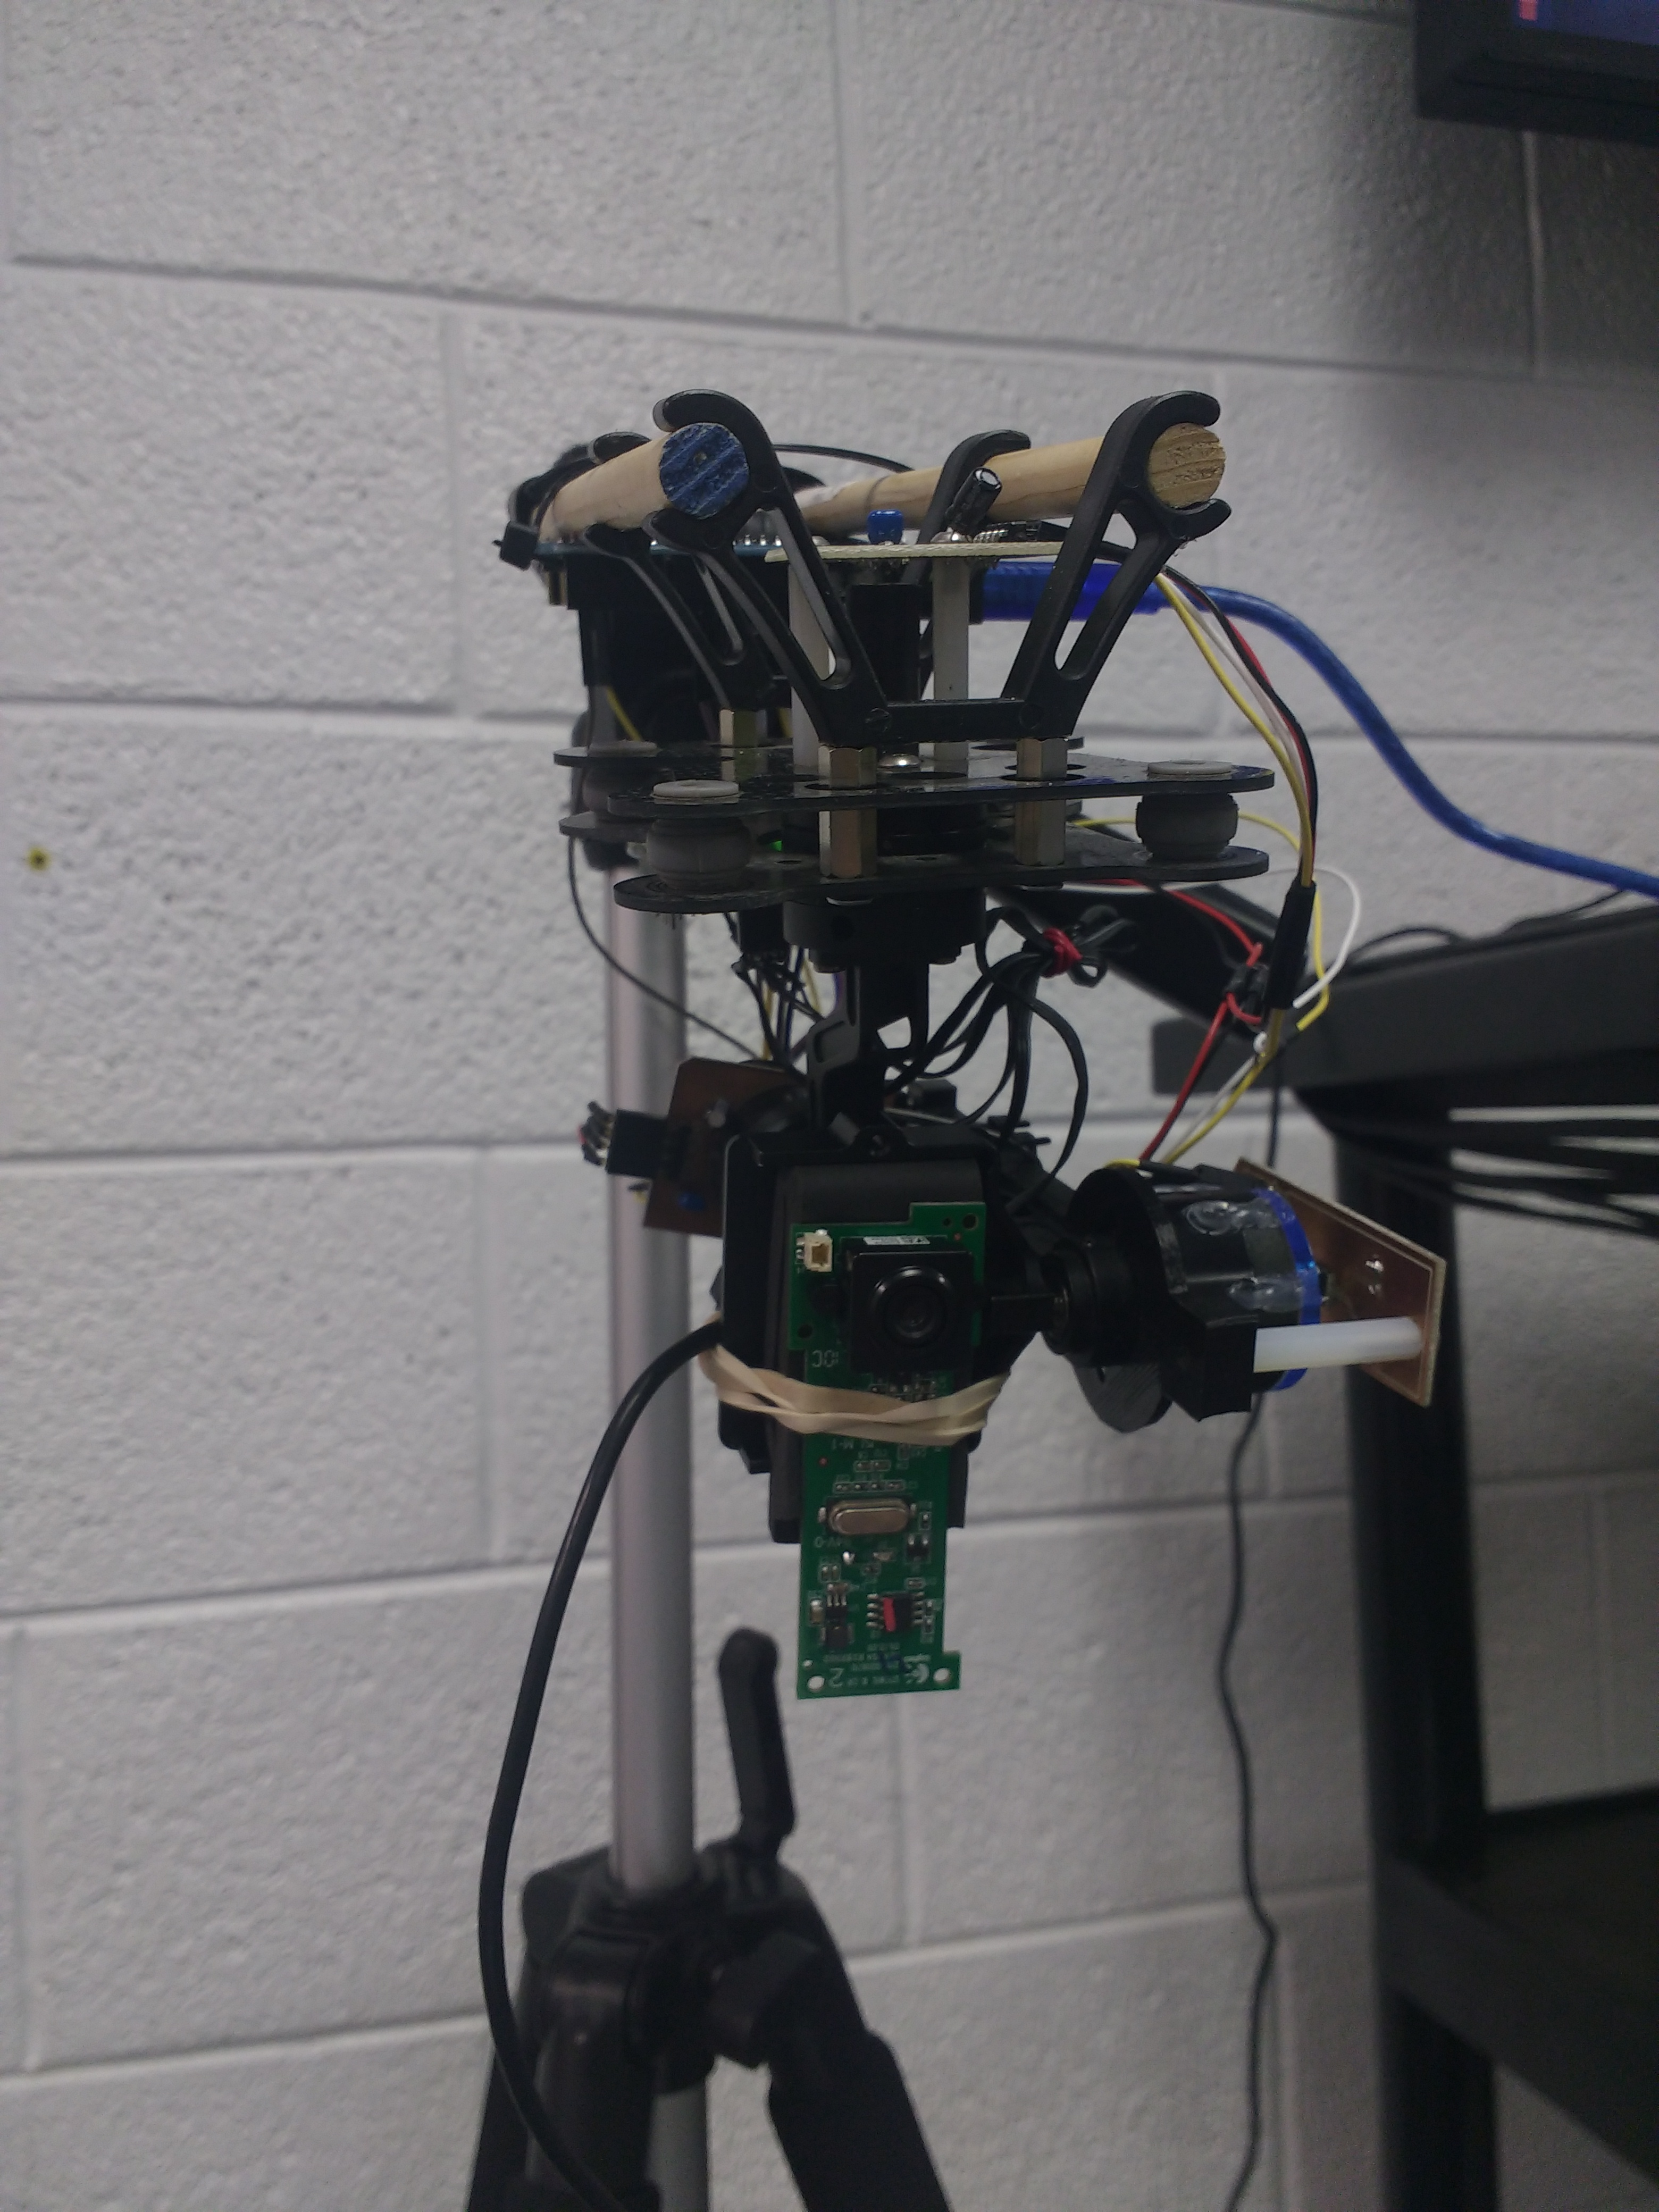
\includegraphics[width = 3in]{images/chapter2/gimbal_webcam.jpg}
	\caption{Prototype hardware to test gimbal control algorithm}
	\label{gimbal_webcam}
\end{figure}
The angle commanding control algorithm has been implemented and tested with simple hardware (see Figure \ref{gimbal_webcam}). The major hardware component includes BaseCam SimpleBGC 32-bit gimbal controller, a webcam, DYS 3-axis GoPro gimbal, and AS5048B magnetic rotary encoder attached to each rotating axis to get the exact gimbal angles. Note that in this hardware experiment, the roll axis of gimbal is always commanded to be zero to pan-tilt camera gimbal. The focal length of camera is known through the camera calibration process and the target pixel location is given by the color detection algorithm implemented using OpenCV \cite{itseez2015opencv}. The gimbal control algorithm is keeping the target, a line following ground robot, at the center of the camera field of view (see Figure \ref{gimbal_result}. Also, the result video can be found at \href{https://www.youtube.com/watch?v=OZ0Mg8AoAzk}{https://www.youtube.com/watch?v=OZ0Mg8AoAzk}). 

\begin{figure*}[t]
	\centering
	\begin{subfigure}{0.5\textwidth}
		\centering
		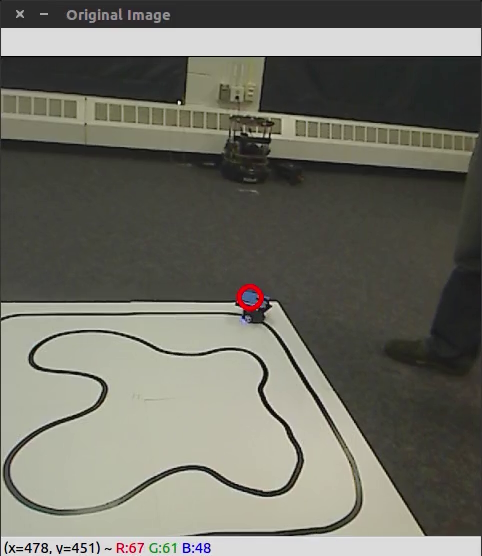
\includegraphics[width=0.7\linewidth]{images/chapter2/gimbal_0s.png}
		\caption{when $t=0s$}
	\end{subfigure}%
	\begin{subfigure}{0.5\textwidth}
		\centering
		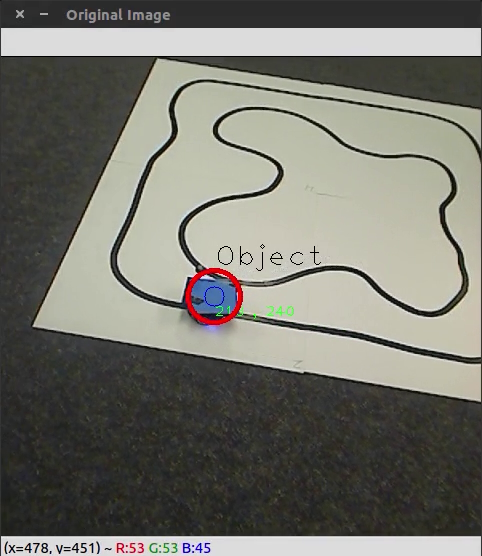
\includegraphics[width=0.7\linewidth]{images/chapter2/gimbal_10s.png}
		\caption{when $t=10s$}
	\end{subfigure}
	\begin{subfigure}{0.5\textwidth}
		\centering
		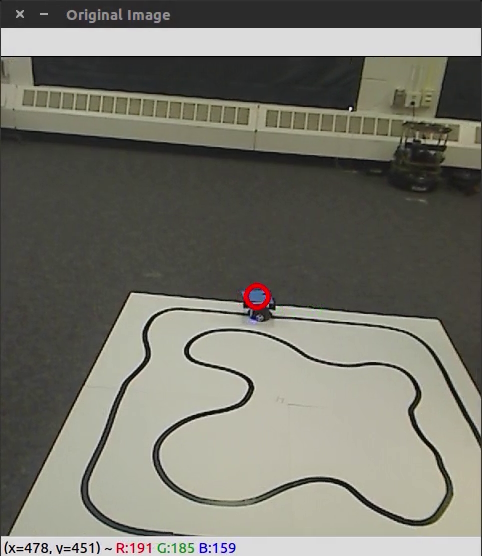
\includegraphics[width=0.7\linewidth]{images/chapter2/gimbal_20s.png}
		\caption{when $t=20s$}
	\end{subfigure}%
	\begin{subfigure}{0.5\textwidth}
		\centering
		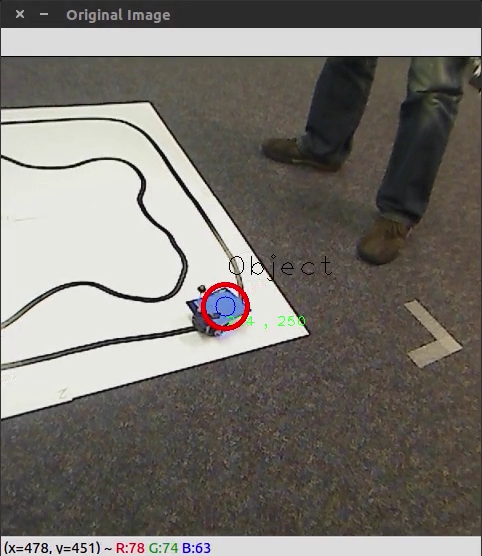
\includegraphics[width=0.7\linewidth]{images/chapter2/gimbal_30s.png}
		\caption{when $t=30s$}
	\end{subfigure}
	\begin{subfigure}{0.5\textwidth}
		\centering
		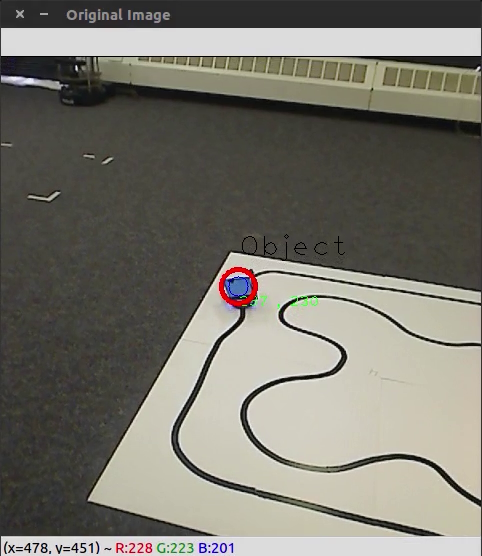
\includegraphics[width=0.7\linewidth]{images/chapter2/gimbal_40s.png}
		\caption{when $t=40s$}
	\end{subfigure}	
	\caption{Hardware demonstration. The gimbal control algorithm is keeping the target object at the center of the camera field of view.}
	\label{gimbal_result}
\end{figure*}


\section{Angular Velocity Commanding Gimbal Control}
In the previous section, a relatively simple gimbal control algorithm is presented. One disadvantage of it is that it does not take the camera velocity into consideration. When gimbal is mounted on a stationary platform, the angle commanding controller can perform without any performance degradation. However, if the gimbal is mounted on UAV, taking the camera velocity into account in the controller becomes important. The work in \cite{Hurak2012} addresses this issue and derives the control algorithm that overcomes the issue. This angular velocity commanding gimbal control algorithm is presented briefly in this section because some of the concepts in this section introduces important background for the next section. 

\begin{figure}[t]
	\centering
	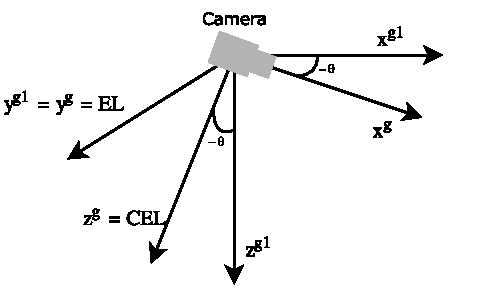
\includegraphics[width = 3in]{images/chapter2/cross_elevation.pdf}
	\caption{Elevation and cross-elevation axis}
	\label{cross_elevation}
\end{figure}
\subsection{Image Jacobian}
A full derivation of getting Image Jacobian matrix (often called interaction matrix) can be found in \cite{spong2006robot}. Here, we only show the final form of Image Jacobian in the process of developing the gimbal control algorithm. Let the camera translational and rotational velocities both expressed in the camera frame be defined as
\begin{equation}
\mathbf{v}_C=[v_{Cx}, v_{Cy}, v_{Cz}]^\top
\end{equation}
\begin{equation}
\mathbf{\omega}_C=[\omega_{Cx}, \omega_{Cy}, \omega_{Cz}]^\top
\end{equation}
\begin{equation}
\mathbf{\xi}=[\mathbf{v}_C^\top, \mathbf{\omega}_C^\top]^\top.
\label{camera_velocity}
\end{equation}
In this section, $[A]$ stands for azimuth frame, $[E]$ stands for elevation frame, and $[C]$ stands for camera frame (see Figure \ref{cross_elevation}). $\theta$ indicates the elevation angle and $\psi$ indicates the azimuth angle. Also, following the convention in Figure \ref{camera_frame}, 
\begin{equation}
R^{E}_C =
\begin{bmatrix}
0 & 0 & 1 \\
1 & 0 & 0 \\
0 & 1 & 0
\end{bmatrix}.
\end{equation}
Also, let the coordinates of image feature and its velocity can be defined as 
\begin{equation}
\mathbf{s}=[u, w]^\top
\end{equation}
and 
\begin{equation}
\mathbf{\dot{s}}=[\dot{u}, \dot{w}]^\top.
\label{image_feature_velocity}
\end{equation}
Image Jacobian matrix $L$ shows the relationship between the camera velocity in (\ref{camera_velocity}) and the image feature velocity in (\ref{image_feature_velocity}) and can be expressed as 
\begin{equation}
\mathbf{\dot{s}}=L(\mathbf{s},z,\lambda)\mathbf{\xi}
\end{equation}
or more explicitly
\begin{equation}
\begin{bmatrix}
\dot{u} \\ \dot{w}
\end{bmatrix}
=\begin{bmatrix}
-\frac{\lambda}{z} & 0 & \frac{u}{z} & \frac{uw}{\lambda} & -\frac{\lambda^2+u^2}{\lambda} & w \\
0 & -\frac{\lambda}{z} & \frac{w}{z} & \frac{\lambda^2+w^2}{\lambda} & -\frac{uw}{\lambda} & -u
\end{bmatrix}
\begin{bmatrix}
v_{Cx} \\ v_{Cy} \\ v_{Cz} \\
\omega_{Cx} \\ \omega_{Cy} \\ \omega_{Cz}
\end{bmatrix}
\label{image_jacobian}
\end{equation}
where $z$ is the depth along the optical axis to where the target lies and $\lambda$ is the focal length. Note that $\lambda$ is a fixed parameter once the camera is calibrated. The equation (\ref{image_jacobian}) can be divided into two parts: one for the camera translational velocity and the other for rotational velocity as
\begin{align}
\mathbf{\dot{s}}&=\begin{bmatrix}
-\frac{\lambda}{z} & 0 & \frac{u}{z} \\
0 & -\frac{\lambda}{z} & \frac{w}{z}
\end{bmatrix}\mathbf{v}_C+
\begin{bmatrix}
\frac{uw}{\lambda} & -\frac{\lambda^2+u^2}{\lambda} & w \\
\frac{\lambda^2+w^2}{\lambda} & -\frac{uw}{\lambda} & -u
\end{bmatrix}\mathbf{\omega}_C
\\&=L_v(u,w,z)\mathbf{v}_C+L_{\omega}(u,w)\mathbf{\omega}_C
\label{image_jacobian1}
\end{align}
It is worth to note that only the translational part depends on the target depth $z$. 

\subsection{Feedback Linearization-based Visual Pointing and Tracking}
The controller's objective is to drive an image feature to the center of image. The horizontal error can be eliminated by moving two axis gimbal motors attached on azimuth and elevation axis. Moving only the azimuth axis can not compensate for the horizontal error because it only indirectly affects $E_z$ axis which is often referred as cross-elevation axis $CEL$. Thus, some vertical error is introduced and it needs to be compensated by moving the elevation at next time step. However, the key idea of the controller is that exploiting $\omega_{Ex}$ term in a clever way we can find the azimuth and elevation commands for the same time step that smoothly compensate for the horizontal error without introducing the vertical error. Let the error in the image plane be
\begin{equation}
e(t)=s(t)-s^{ref}
\label{image_feature_error}
\end{equation}
where $s^{ref}=[0, 0]^\top$ to push the image feature to the image center. We would like to derive (\ref{image_feature_error}) to zeros by controlling $\omega_{EL}=\omega_{Ey}$ and $\omega_{AZ}=\frac{\omega_{Ez}}{\cos \theta}$. Manipulating the equation (\ref{image_jacobian1}) gives
\begin{equation}
L_{\omega}(u,w)\mathbf{\omega}_C=\dot{s}-L_v(u,w,z)\mathbf{v}_C.
\label{image_jacobian2}
\end{equation}
Note that our interest is to find camera angular rate command only and camera translational rate can be measured when UAV is flying independent from the gimbal controller. The null space of the matrix $L_{\omega}$ can be parameterized as
\begin{equation}
N(L_{\omega})=\{\omega_C=k\begin{bmatrix}
u & w & \lambda
\end{bmatrix}^\top\}
\label{nullspace}
\end{equation}
and adding (\ref{nullspace}) to (\ref{image_jacobian2}) makes
\begin{equation}
L_{\omega}(u,w)\mathbf{\omega}_C=\dot{s}-L_v(u,w,z)\mathbf{v}_C+L_{\omega}(u,w)k\begin{bmatrix}
u \\ w \\ \lambda
\end{bmatrix}.
\label{image_jacobian3}
\end{equation}
This null space means that rotation about the axis connecting the image feature and the origin of optical axis do not change the coordinates of the image feature. The left pseudoinverse of $L_{\omega}$ is given by 
\begin{equation}
L_{\omega}^\sharp=\begin{bmatrix}
0 & \frac{\lambda}{\lambda^2+u^2+w^2} \\
-\frac{\lambda}{\lambda^2+u^2+w^2} & 0 \\
\frac{w}{\lambda^2+u^2+w^2} & -\frac{u}{\lambda^2+u^2+w^2}
\end{bmatrix}
\label{pseudoinverse}
\end{equation}
and multiplying both side of (\ref{image_jacobian3}) by (\ref{pseudoinverse}) yields
\begin{equation}
\mathbf{\omega}_C=\frac{1}{z(\lambda^2+u^2+w^2)}\begin{bmatrix}
\lambda^2 v_y-\lambda v_z w+\lambda \dot{w}z+ku \\
-\lambda^2 v_x+\lambda v_zu-\lambda \dot{u}z+kw \\
-\lambda u v_y+\lambda w v_x-u\dot{w}z+\dot{u}wz+k\lambda
\end{bmatrix}.
\label{angular_rate}
\end{equation}
If we require $\dot{s}^{ref}(t)=-\alpha Is(t)$ where $\alpha$ is a positive value, the actual value of $s(t)$ is expected to be exponentially stable which means it converges to zero. Thus, 
\begin{equation}
\mathbf{\dot{s}}^{ref}=\begin{bmatrix}
\dot{u}^{ref} \\ \dot{w}^{ref}
\end{bmatrix}
=-\alpha \begin{bmatrix}
1 & 0 \\ 0 & 1
\end{bmatrix}
\begin{bmatrix}
u \\ w
\end{bmatrix}
=\begin{bmatrix}
-\alpha u \\ -\alpha w
\end{bmatrix}.
\label{sdot_reference}
\end{equation}
By plugging the equation (\ref{sdot_reference}) into (\ref{angular_rate}), we can compute the desired camera angular rate that guarantees the asymptotic stability for the image error as
\begin{equation}
\mathbf{\omega}_C^{ref}=\frac{1}{z(\lambda^2+u^2+w^2)}\begin{bmatrix}
\lambda^2 v_y-\lambda v_z w -\lambda \alpha wz+ku \\
-\lambda^2 v_x+\lambda v_zu +\lambda \alpha uz+kw \\
-\lambda u v_y+\lambda w v_x +k\lambda
\end{bmatrix}.
\label{angular_rate_reference}
\end{equation}
This angular rate reference commands expressed in the camera frame must be transformed into the elevation frame in order to make them direct command for each gimbal axis as
\begin{align}
\mathbf{\omega}_E^{ref}&=R_C^E\mathbf{\omega}_C^{ref}
=\begin{bmatrix}
\omega_{Ex}^{ref} \\ \omega_{Ey}^{ref} \\ \omega_{Ez}^{ref}
\end{bmatrix}
\\&=\frac{1}{z(\lambda^2+u^2+w^2)}\begin{bmatrix}
-\lambda u v_y+\lambda w v_x +k\lambda \\
\lambda^2 v_y-\lambda v_z w -\lambda \alpha wz+ku \\
-\lambda^2 v_x+\lambda v_zu +\lambda \alpha uz+kw \\
\end{bmatrix}.
\label{angular_rate_ref_elevation}
\end{align}
It is questionable that $\mathbf{\omega}_C^{ref}$ has commands for three axis, but there are only two controllable axis, namely $\omega_{Ey}$ and $\omega_{Ez}$. This problem can be solved by using the free parameter $k$ to come up with two proper motor commands. The key strategy of picking $k$ is to select the $k$ value that does not require any change from the current $\omega_{Ex}$ value as 
\begin{equation}
k=uv_y-wv_x+\frac{z(\lambda^2+u^2+w^2)}{\lambda}\omega_{Ex}
\label{k}
\end{equation}
which indicates that $\omega_x$ must be measured from a sensor such as MEMS gyro attached to the camera. Substituting for $k$ in $\omega_{Ey}^{ref}$ and $\omega_{Ez}^{ref}$ from the equation (\ref{angular_rate_ref_elevation}) with (\ref{k}) gives
\begin{equation}
\omega_{EL}^{ref}=\omega_{Ey}^{ref}=\frac{\lambda^2 v_y-\lambda v_z w -\lambda \alpha wz+u^2 v_y-uwv_x}{z(\lambda^2+u^2+w^2)}+\frac{\omega_{Ex}u}{\lambda}
\end{equation}
\begin{equation}
\omega_{CEL}^{ref}=\omega_{Ez}^{ref}=\frac{-\lambda^2 v_x+\lambda v_z u+\lambda \alpha uz +uwv_y -w^2 v_x}{z(\lambda^2+u^2+w^2)}+\frac{\omega_{Ex}w}{\lambda}.
\end{equation}
Using the relationship 
\begin{equation}
\omega_{AZ}=\frac{1}{\cos\theta}\omega_{CEL},
\end{equation}
we can compute the desired angular rate on azimuth axis instead of cross-elevation axis as
\begin{equation}
\omega_{AZ}^{ref}=\frac{1}{\cos \theta}\bigg(\frac{-\lambda^2 v_x+\lambda v_z u+\lambda \alpha uz +uwv_y -w^2 v_x}{z(\lambda^2+u^2+w^2)}+\frac{\omega_{Ex}w}{\lambda}\bigg).
\end{equation}
\begin{figure}[t]
	\centering
	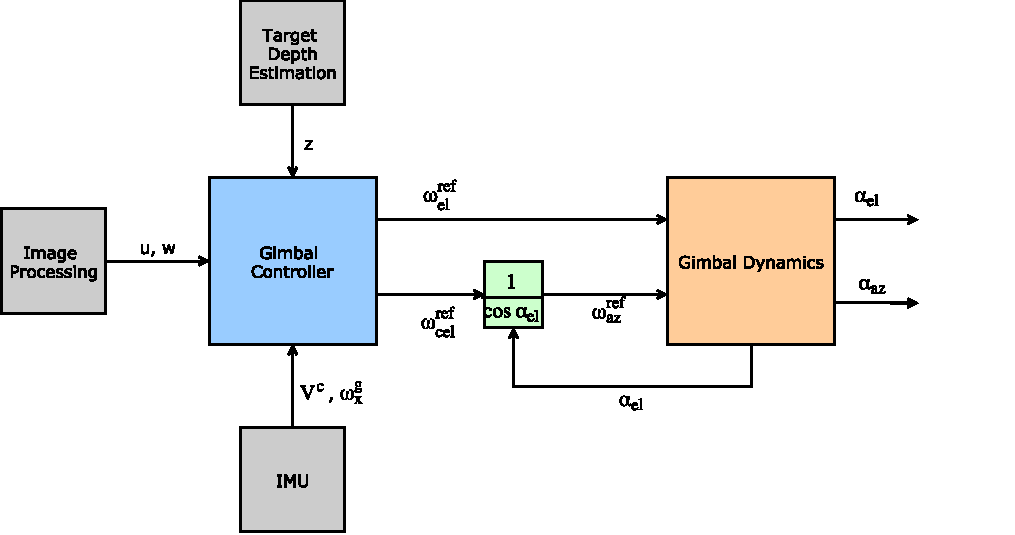
\includegraphics[width = 5in]{images/chapter2/gp_blockdiagram.pdf}
	\caption{Angular velocity commanding gimbal controller block diagram}
	\label{avcg_blockdiagram}
\end{figure}
The system block diagram of this controller can be found in Figure \ref{avcg_blockdiagram}. The controller presents the ideal control scheme for two axis inertially stabilized gimbal system, but it also presents some technical challenges such as estimating the depth to the target or estimating the camera translational velocity. The camera translational velocity can be either estimated by using the UAV velocity if available or be treated as disturbance. Estimating the depth can be handled using a laser range finder if available or geolocation technique or adaptive depth gimbal control algorithm which is elaborated in the next section.

\section{Adaptive Depth Gimbal Control}
The gimbal control algorithm in the previous section provides with a great way to keep a target of interest in the camera's field of view with gimbal azimuth and elevation incorporating control effort rather than decoupled controls for azimuth and elevation separately. On top of the framework established in the previous section, this section examines a way to remove the necessity of externally feeding the depth, $z$ term in the Image Jacobian equation (\ref{image_jacobian}). Instead, the controller estimates the depth online as a part of the controller while the control objective of pointing to the target is still being accomplished. This controller is inspired by a non-linear adaptive control technique called Model Reference Adaptive Control (MRAC).
\subsection{Introduction}
!!!!!!!!!!!!!!!!! HERE EXPLAIN MRAC BRIEFLY !!!!!!!!!
\subsection{Derivation}
Let's revisit the Image Jacobian matrix
\begin{equation}
\begin{bmatrix}
\dot{u} \\ \dot{w}
\end{bmatrix}
=\begin{bmatrix}
-\frac{\lambda}{z} & 0 & \frac{u}{z} & \frac{uw}{\lambda} & -\frac{\lambda^2+u^2}{\lambda} & w \\
0 & -\frac{\lambda}{z} & \frac{w}{z} & \frac{\lambda^2+w^2}{\lambda} & -\frac{uw}{\lambda} & -u
\end{bmatrix}
\begin{bmatrix}
v_{Cx} \\ v_{Cy} \\ v_{Cz} \\
\omega_{Cx} \\ \omega_{Cy} \\ \omega_{Cz}
\end{bmatrix}
\end{equation}
or for simplicity
\begin{equation}
\mathbf{\dot{s}}=L_v(u,w,z)\mathbf{v}_C+L_{\omega}(u,w)\mathbf{\omega}_C.
\end{equation}
Since we desire that the target is pushed to the center of image plane, the reference model can be set as 
\begin{equation}
\mathbf{\dot{s}}^{ref}=A_{ref}\mathbf{s}^{ref}
\label{reference_model}
\end{equation}
where $\mathbf{s}=[u, w]^\top$ and $A^{ref}$ is Hurwitz or every eigenvalue of $A^{ref}$ has strictly negative real part. It is clear that the reference model in (\ref{reference_model}) is globally asymptotically stable. Manipulating the Image Jacobian matrix to be in more convenient form to develop the adaptive controller yields 